\subsection{Conflict Detection}

\begin{frame}{Collision Detection Schemes}
The primary rationale for an automated intersection is to prevent traffic accidents.
Methods to predict collisions:
\begin{itemize}
\item Tiling -- Autonomous Intersection Management (AIM) project at UT Austin
\item Euclidean distance between three-dimensional trajectories $f(x,\,y,\,t)$
\end{itemize}
We would like an alternative that is less computationally intensive
and amenable to optimization.
\end{frame}

\begin{frame}{Conflict Points}
\begin{definition}
A \emph{traffic conflict point} is the point at which multiple
	traffic flows may cross or merge.
\end{definition}
\begin{itemize}
\item Require that all vehicles adhere to designated lanes when
	traversing the intersection, so that trajectories can be bounded
	exactly.
\item The set of conflict points are determined by the intersections
	between curves representing all legal paths of vehicles.
\end{itemize}
\end{frame}

%%

\begin{frame}{Intersection Geometry}
\begin{itemize}
\item Four-way symmetric intersection with orthogonal arms and
	perfect alignment
\item Open space without obstructions (e.g., channelization
	features, pedestrians)
\item Total number of lanes at any exit approach equals the
	total number of lanes at any entrance approach
\item Traffic lanes at an exit approach can only serve as the
	exit of lanes with the same lane number relative to
	the center line
\item No exclusive right/left turn lanes
\end{itemize}
\end{frame}

%%

\begin{frame}{Path Equations}
\begin{tabular}{c l}
$N$ & number of lanes per direction \\
$M$ & number of left turn lanes per direction ($M < N$) \\
$w$ & lane width \\
$c$ & corner radius \\
$d$ & minimum buffer distance between vehicles in potential conflict \\
$k$ & lane number \\
\end{tabular}

\vspace{\baselineskip}
Quantities defined for convenience:
\begin{align*}
\alpha_k &= \left(k - \frac{1}{2}\right) w
	& \text{\scriptsize offset from center line} \\
\beta_k &= \frac{1}{\sqrt{2}} \left[ \frac{d}{2} +
	\left(M - k + \frac{1}{2}\right) w \right]
	& \text{\scriptsize projected offset from origin} \\
\gamma &= N w + c & \text{\scriptsize half of intersection width}
\end{align*}
\end{frame}

%%

\begin{frame}{Path Equations}
\begin{itemize}
\item Straight:
\end{itemize}
	\begin{align}
	y &= \pm \alpha_k & k = 1,\dots,N \\
	x &= \pm \alpha_k & k = 1,\dots,N
	\end{align}

\begin{itemize}
\item Right turns: Circular quadrants of radius $\frac{w}{2} + c$ ($k = M + 1,\dots,N$)
\end{itemize}
	\begin{center}
	\begin{tabular}{c|c c c}
	Direction & Center & Entrance & Exit \\
	\hline
	$\text{S} \to \text{E}$ & ($\gamma$, $-\gamma$) & ($\alpha_k$, $-\gamma$) & ($\gamma$, $-\alpha_k$) \\
	$\text{N} \to \text{W}$ & ($-\gamma$, $\gamma$) & ($-\alpha_k$, $\gamma$) & ($-\gamma$, $\alpha_k$) \\
	$\text{E} \to \text{N}$ & ($\gamma$, $\gamma$) & ($\gamma$, $\alpha_k$) & ($\alpha_k$, $\gamma$) \\
	$\text{W} \to \text{S}$ & ($-\gamma$, $-\gamma$) & ($-\gamma$, $-\alpha_k$) & ($-\alpha_k, -\gamma$) \\
	\end{tabular}
	\end{center}

\end{frame}

%%

\begin{frame}{Path Equations: Left Turns}
\begin{itemize}
\item Circular arcs fitted to three control points ($k = 1,\dots,M$):
\end{itemize}
	\begin{center}
	\begin{tabular}{c|c c c}
	Direction & Entrance & Midpoint & Exit \\
	\hline
	$\text{S} \to \text{W}$ & ($\alpha_k$, $-\gamma$) & ($-\beta_k$, $-\beta_k$) & ($-\gamma$, $\alpha_k$) \\
	$\text{N} \to \text{E}$ & ($-\alpha_k$, $\gamma$) & ($\beta_k$, $\beta_k$) & ($\gamma$, $\alpha_k$) \\
	$\text{E} \to \text{S}$ & ($\gamma$, $\alpha_k$) & ($\beta_k$, $-\beta_k$) & ($-\alpha_k$, $-\gamma$) \\
	$\text{W} \to \text{N}$ & ($-\gamma$, $-\alpha_k$) & ($-\beta_k$, $\beta_k$) & ($\alpha_k$, $\gamma$) \\
	\end{tabular}
	\end{center}
\begin{itemize}
\item Outermost left turn lane is diagonally offset $\frac{d + w}{2}$ from
origin to avoid conflicts with oncoming left turn traffic.
\item For simplicity, U-turns are disallowed.
\end{itemize}
\end{frame}

%%

\begin{frame}{Circumcircle of a Triangle}
	\begin{align*}
	a &= \phantom{-}\begin{vmatrix}
	x_1 & y_1 & 1 \\
	x_2 & y_2 & 1 \\
	x_3 & y_3 & 1
	\end{vmatrix} &
	b_x &= -\begin{vmatrix}
	\left( x_1^2 + y_1^2 \right) & y_1 & 1 \\
	\left( x_2^2 + y_2^2 \right) & y_2 & 1 \\
	\left( x_3^2 + y_3^2 \right) & y_3 & 1 \\
	\end{vmatrix} \\
	c &= -\begin{vmatrix}
	\left( x_1^2 + y_1^2 \right) & x_1 & y_1 \\
	\left( x_2^2 + y_2^2 \right) & x_2 & y_2 \\
	\left( x_3^2 + y_3^2 \right) & x_3 & y_3 \\
	\end{vmatrix} &
	b_y &= \phantom{-}\begin{vmatrix}
	\left( x_1^2 + y_1^2 \right) & x_1 & 1 \\
	\left( x_2^2 + y_2^2 \right) & x_2 & 1 \\
	\left( x_3^2 + y_3^2 \right) & x_3 & 1 \\
	\end{vmatrix}
	\end{align*}

\begin{minipage}[t]{0.45\linewidth}
	Circumcenter:
	\begin{align}
	x_c &= -\frac{b_x}{2 a} \\
	y_c &= -\frac{b_y}{2 a}
	\end{align}
\end{minipage}
\hfill
\begin{minipage}[t]{0.45\linewidth}
	Circumradius:
	\begin{equation}
	r = \frac{\sqrt{b_x^2 + b_y^2 - 4 a c}}{2 |a|}
	\end{equation}
\end{minipage}
\end{frame}

%%

\begin{frame}{Conflict Points of Model Intersection}
\centering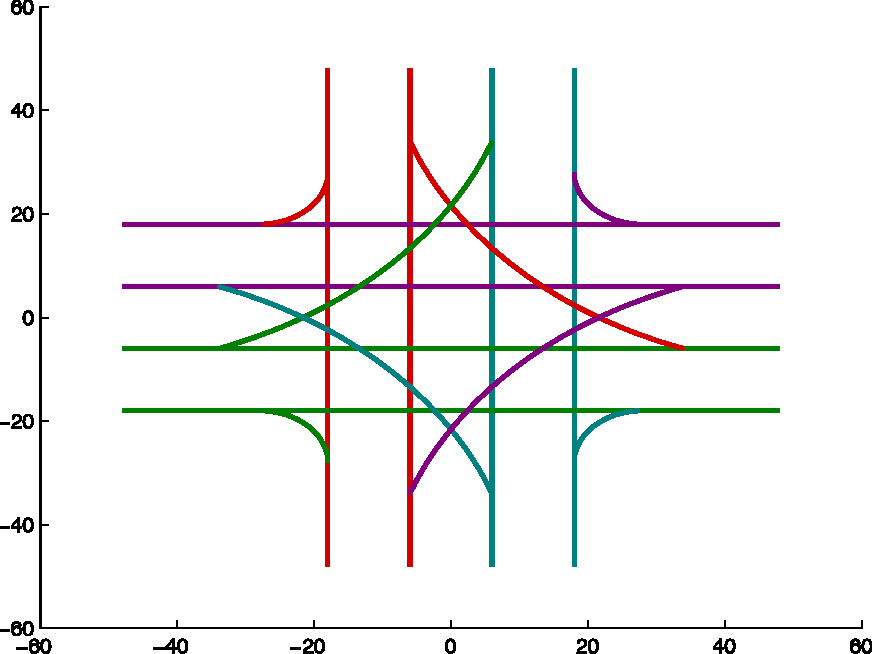
\includegraphics[width=0.8\linewidth]{diagram/intxn_plain.pdf}
\end{frame}

%%

\begin{frame}{Conflict Points of Model Intersection}
\centering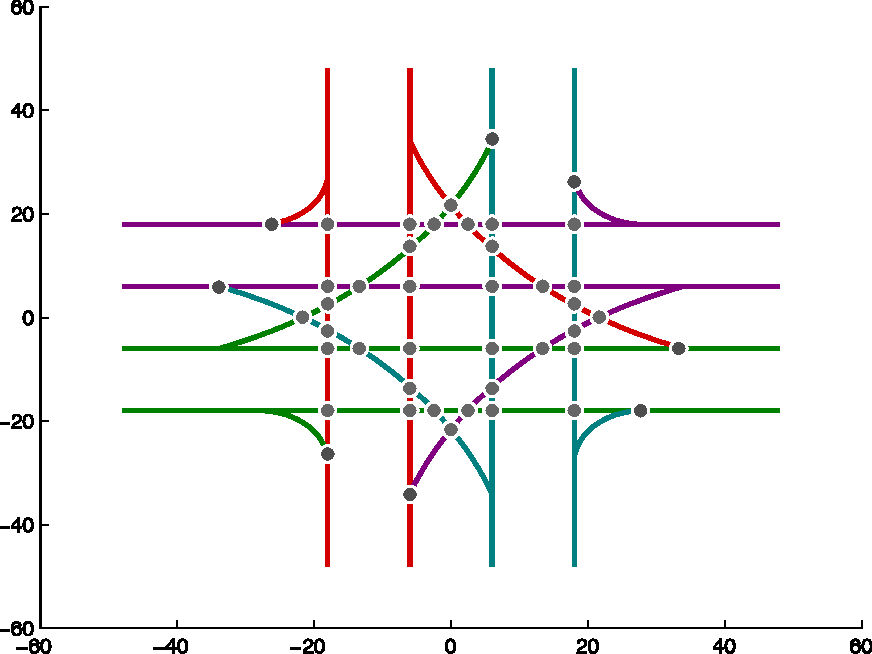
\includegraphics[width=0.8\linewidth]{diagram/intxn_pts.pdf}
\end{frame}

%%

\begin{frame}{Conflict Zones}
\begin{itemize}
\item In reality, vehicles are not point masses -- they occupy area.
\item \textbf{Safety property}:
	Enforce a minimum separation distance $d$ at all times
	between vehicles traveling on conflicting paths.
\end{itemize}

\begin{definition}
A \emph{traffic conflict zone} is the segment of a given path within
	distance $d$ of a conflict point.
\end{definition}

\begin{itemize}
\item The initial and terminal points of a conflict zone can be expressed
	as an ordered pair of offsets/displacements along the curve, relative
	to the start of the path.
\end{itemize}
\end{frame}

%%

\begin{frame}{Position as Arc Length}
\begin{itemize}
\item Recall that all turns are modeled as circular arcs.
\item Central angle with vertex ($x_c$, $y_c$), endpoint ($x$, $y$)
	on the circle, and one side parallel to the x-axis:
\end{itemize}
\begin{equation}
\theta(x, y) = \left| \arccos\left(\frac{x - x_c}{r}\right) \right|
	= \left| \arcsin\left(\frac{y - y_c}{r}\right) \right|
\end{equation}

\begin{itemize}
\item Arc length (displacement) from the initial point ($x_0$, $y_0$)
	to the terminal point ($x_1$, $y_1$):
\end{itemize}
\begin{equation}
s = r |\theta(x_1, y_1) - \theta(x_0, y_0)|
\end{equation}

\begin{itemize}
\item Only one coordinate needs to be known for each endpoint.
\end{itemize}
\end{frame}

%%

\begin{frame}{Conflict Point Displacements}
\begin{itemize}
\item $w = 12$ ft, $c = 10$ ft, $d = 15$ ft
\item Merge conflict points (highlighted in {\color{red} red})
	are the exit points of turns, which also indicate the total
	length of each path.
\end{itemize}

\begin{center}
\scriptsize\setlength{\tabcolsep}{3pt}
	\begin{tabular}{| c | c c c c | c c c c | c c c c |}
	\multicolumn{1}{c}{}
		& \multicolumn{4}{c}{\large $\longrightarrow$}
		& \multicolumn{4}{c}{\large $\downarrow$}
		& \multicolumn{4}{c}{\large $\longleftarrow$} \\
	\hline
	{}
		& L & S1 & S2 & R
		& L & S1 & S2 & R
		& L & S1 & S2 & R \\
	\hline
	L
		& 44.62 & 34.44 & 18.12 & --
		&   --   & 23.99 & 40.30 & --
		& 13.80 & {\color{red} 58.42} & -- & -- \\
	S1
		& -- & 28.00 & 16.00 & --
		& 47.38 & -- & -- & --
		& 20.62 & 40.00 & 52.00 & {\color{red} 68.00} \\
	S2
		& {\color{red} 68.00} & 28.00 & 16.00 & --
		& 36.39 & -- & -- & --
		& 31.61 & 40.00 & 52.00 & -- \\
	R
		& -- & -- & {\color{red} 25.13} & --
		& -- & -- & -- & --
		& -- & -- & -- & -- \\
	\hline
	\end{tabular}
\end{center}
\end{frame}

%%

\begin{frame}{Conflict Zone Partitioning}
Rigorous method is to calculate intersection points between a circle
of radius $d$, centered at conflict point ($x$, $y$), and involved
path curves -- more complicated than necessary.

\begin{itemize}
\item Conflict zones for straight paths are simply $x \pm d$ for
	$\text{E} \rightleftarrows \text{W}$ and $y \pm d$ for
	$\text{N} \rightleftarrows \text{S}$.
\item The chord length approximates the circular arc length when the
	subtended angle remains relatively small.  For left turns where
	$d \ll r$, the extent of a conflict zone can be treated as $s \pm d$.
\item The entire right turn path is considered a conflict zone.
%\item For right turns, the initial point of the conflict zone is
%	$[ \frac{1}{4}\pi - 2\arcsin(\frac{d}{2 c}) ] c$.
\end{itemize}
\textbf{Aggregation}: Group conflict points into multiple overlapping zones
	for coverage and flexibility
\end{frame}

%%

\begin{frame}{Conflict Zone Aggregation}
\centering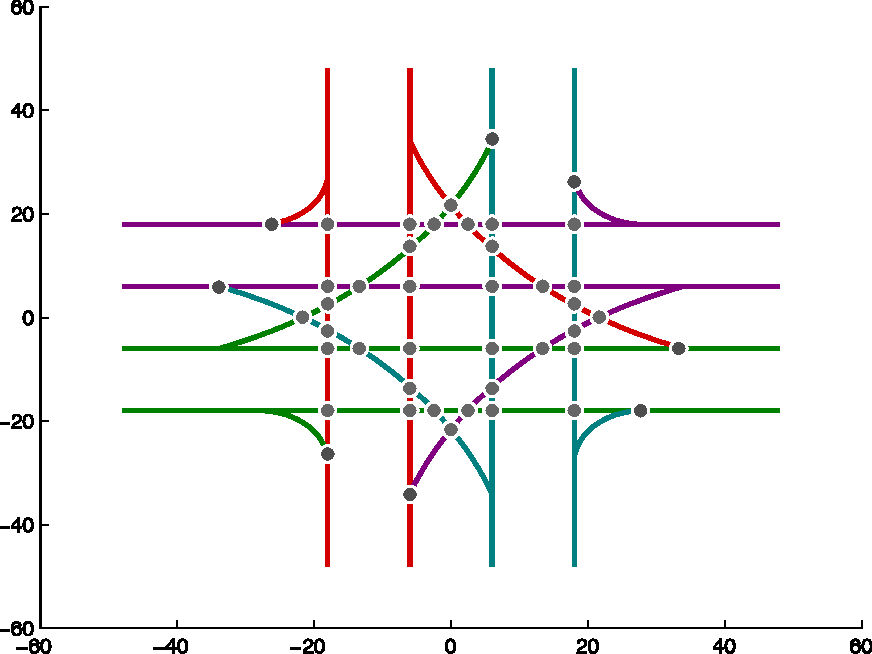
\includegraphics[width=0.8\linewidth]{diagram/intxn_pts.pdf}
\end{frame}

%%

\begin{frame}{Conflict Zone Aggregation}
\centering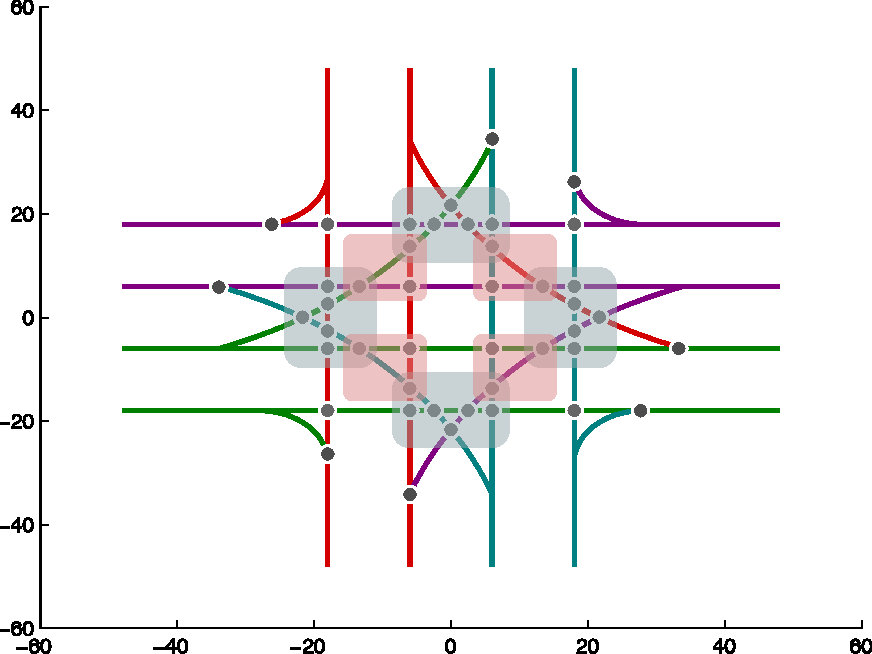
\includegraphics[width=0.8\linewidth]{diagram/intxn_zones.pdf}
\end{frame}

%%

\begin{frame}{Left Turn Path}
\begin{minipage}{0.65\linewidth}
\centering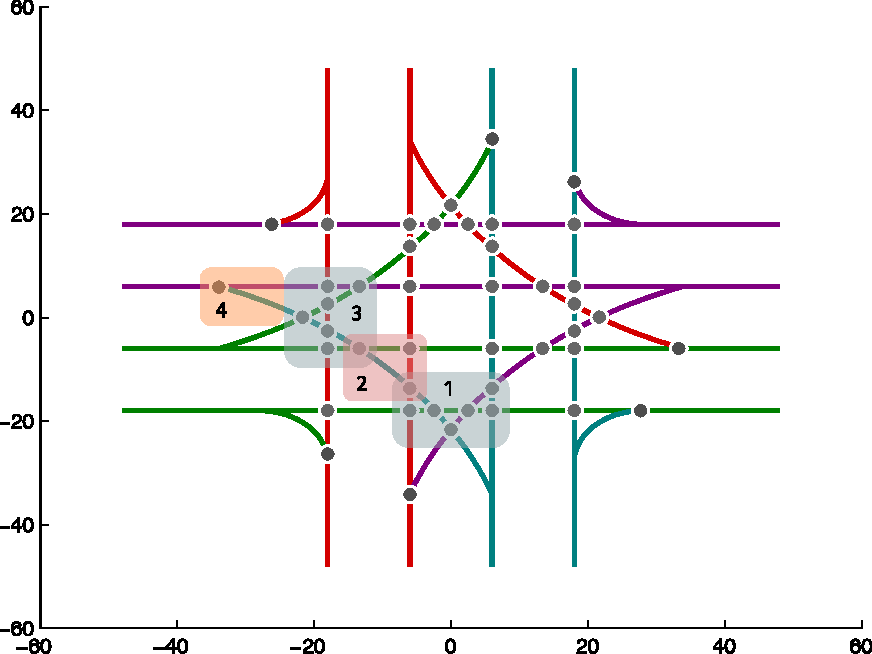
\includegraphics[width=\linewidth]{diagram/intxn_partition_left.pdf}
\end{minipage}
\hfill
\begin{minipage}{0.3\linewidth}
\footnotesize
	\begin{tabular}{| c | r r |}
	\hline
	1 & 8.80 & 28.99 \\
	2 & 18.88 & 39.44 \\
	3 & 29.44 & 49.62 \\
	4 & 43.52 & 58.52 \\
	\hline
	\end{tabular}
\end{minipage}
\end{frame}

%%

\begin{frame}{Straight Path (Inner)}
\begin{minipage}{0.65\linewidth}
\centering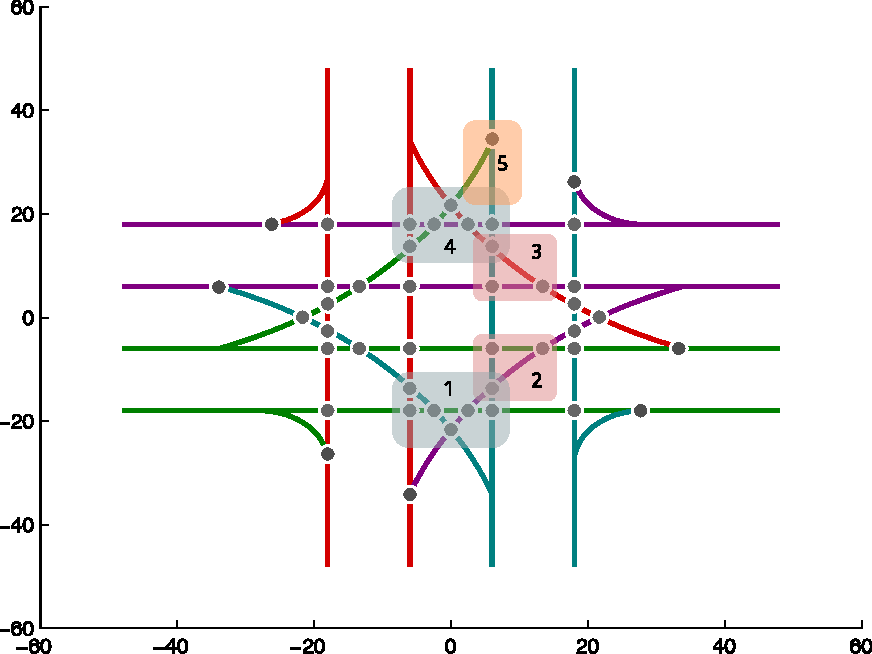
\includegraphics[width=\linewidth]{diagram/intxn_partition_str1.pdf}
\end{minipage}
\hfill
\begin{minipage}{0.3\linewidth}
\footnotesize
	\begin{tabular}{| c | r r |}
	\hline
	1 & 8.50 & 25.62 \\
	2 & 15.62 & 34.00 \\
	3 & 34.00 & 52.38 \\
	4 & 42.38 & 59.50 \\
	5 & 53.00 & 68.00 \\
	\hline
	\end{tabular}
\end{minipage}
\end{frame}

%%

\begin{frame}{Straight Path (Outer)}
\begin{minipage}{0.65\linewidth}
\centering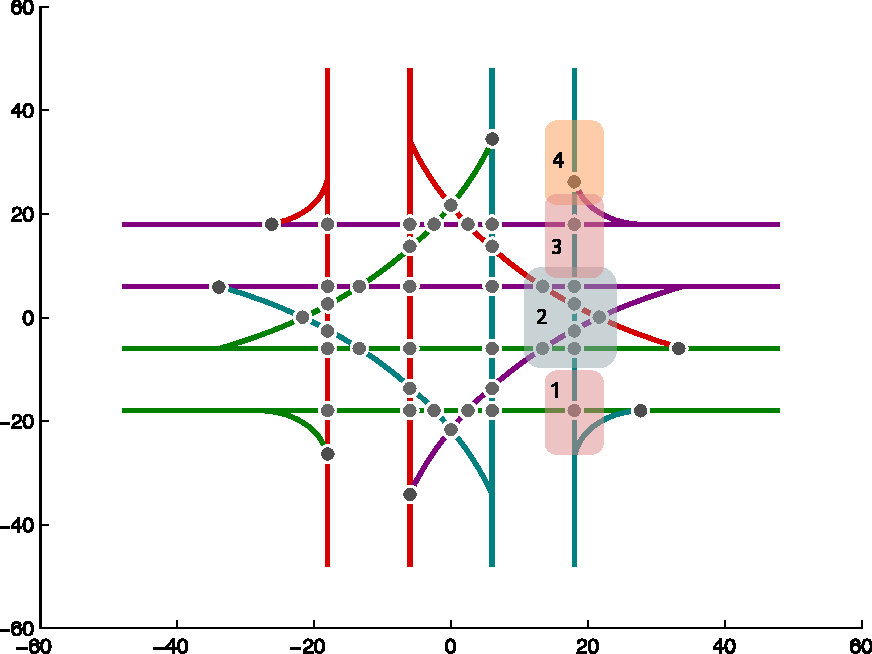
\includegraphics[width=\linewidth]{diagram/intxn_partition_str2.pdf}
\end{minipage}
\hfill
\begin{minipage}{0.3\linewidth}
\footnotesize
	\begin{tabular}{| c | r r |}
	\hline
	1 & 8.50 & 23.50 \\
	2 & 20.50 & 47.50 \\
	3 & 44.50 & 59.50 \\
	4 & 53.00 & 68.00 \\
	\hline
	\end{tabular}
\end{minipage}
\end{frame}

%%

\begin{frame}{Collision Detection Algorithm}
\emph{Given}: Intended route and lane assignment, initial velocity
	$v_0$ at the intersection entrance, planned acceleration function
	$a(t)$, dimensions of vehicle
\begin{enumerate}
\item Determine the set of conflict zones along the path.
\item Numerically integrate to determine when endpoints of conflict
	zones are crossed, yielding a set of time intervals.
\item For each conflict zone, check whether the corresponding time
	interval overlaps with that of any other active vehicle.
\end{enumerate}
\end{frame}

%%

\begin{frame}{Observations}
\begin{itemize}
\item Conflict zones are static and therefore need only to be
	calculated once during initialization.
\item Runtime does not require knowledge about curvature of paths
	-- only linear displacements matter.
\end{itemize}

\begin{block}{Scheduling}
Reservations for a vehicle are scheduled as time intervals during
which it has exclusive access to the conflict zones along its path.
\end{block}

As with majority of other CS problems, finding a solution
is much more difficult than checking a solution.
\end{frame}

\begin{frame}{Questions for Validation}
\begin{itemize}
\item Is it possible for a vehicles with different velocities in the
	same lane to collide without being detected?
	\uncover<2->{
		\begin{itemize}
		\item No, if conflict zones overlap, then the two vehicles
		will be in the same conflict zone when the incident occurs.
		\end{itemize}
	}
\item Are static conflict zones optimal?
	\uncover<2->{
		\begin{itemize}
		\item No, conflict zones must consider worst-case scenarios.
			In reality, vehicles may be at opposite ends of the same
			conflict zone and be sufficiently separated.
		\end{itemize}
	}
\item Can collisions occur at locations other than conflict points?
	\uncover<2->{
		\begin{itemize}
		\item Yes, trajectories can conceivably pass closely together
			but not intersect.  Intersection topology must be designed
			to avoid this.
		\end{itemize}
	}

\end{itemize}
\end{frame}
